\documentclass[12pt]{book}

\newcommand{\thetitle}{Think Java: How to Think Like a Computer Scientist}
\title{\thetitle}

\newcommand{\theauthors}{Allen Downey and Chris Mayfield}
\author{\theauthors}

\newcommand{\theversion}{Version 6.0 Draft -- \today}
\date{\theversion}

\usepackage{geometry}
\geometry{
    width=5.5in,
    height=8.5in,
    hmarginratio=3:2,
    vmarginratio=1:1,
    includehead=true,
    headheight=15pt
}

% paragraph spacing
\setlength{\parindent}{0pt}                      % 17.62482pt
\setlength{\parskip}{12pt plus 4pt minus 4pt}    % 0.0pt plus 1.0pt
\linespread{1.05}
\def\arraystretch{1.5}

% list spacing
\setlength{\topsep}{5pt plus 2pt minus 3pt}      % 10.0pt plus 4.0pt minus 6.0pt
\setlength{\partopsep}{-6pt plus 2pt minus 2pt}  %  3.0pt plus 2.0pt minus 2.0pt
\setlength{\itemsep}{0pt}                        %  5.0pt plus 2.5pt minus 1.0pt

% these are copied from tex/latex/base/book.cls
% all I changed is afterskip
\makeatletter
\renewcommand{\section}{\@startsection {section}{1}{\z@}%
    {-3.5ex \@plus -1ex \@minus -.2ex}%
    {0.7ex \@plus.2ex}%
    {\normalfont\Large\bfseries}}
\renewcommand\subsection{\@startsection{subsection}{2}{\z@}%
    {-3.25ex\@plus -1ex \@minus -.2ex}%
    {0.3ex \@plus .2ex}%
    {\normalfont\large\bfseries}}
\renewcommand\subsubsection{\@startsection{subsubsection}{3}{\z@}%
    {-3.25ex\@plus -1ex \@minus -.2ex}%
    {0.3ex \@plus .2ex}%
    {\normalfont\normalsize\bfseries}}
\makeatother

% table of contents vertical spacing
\usepackage{tocloft}
\setlength\cftparskip{8pt plus 4pt minus 4pt}

% The following line adds a little extra space to the column
% in which the Section numbers appear in the table of contents
\makeatletter
\renewcommand{\l@section}{\@dottedtocline{1}{1.5em}{3.0em}}
\makeatother

% customize page headers
\usepackage{fancyhdr}
\pagestyle{fancyplain}
\renewcommand{\chaptermark}[1]{\markboth{Chapter \thechapter ~~ #1}{}}
\renewcommand{\sectionmark}[1]{\markright{\thesection ~~ #1}}
\lhead[\fancyplain{}{\bfseries\thepage}]%
      {\fancyplain{}{\bfseries\rightmark}}
\rhead[\fancyplain{}{\bfseries\leftmark}]%
      {\fancyplain{}{\bfseries\thepage}}
\cfoot{}
%\rfoot{\textcolor{gray}{\tiny ThinkJava Draft \today}}

% balanced index with TOC entry
\usepackage{makeidx}
\makeindex
%\usepackage[totoc]{idxlayout}

% automatically index glossary terms
\newcommand{\term}[1]{%
\index{#1}
\item[#1:]}
% TODO: doesn't work with plastex
%\newcommand{\term}[1]{\item[#1:]}

% where to find graphics
\usepackage{graphicx}
%\graphicspath{{figs/}}

%% tweak spacing of figures and captions
%\usepackage{floatrow}
%\usepackage{caption}
%\captionsetup{
%    font=small,
%    labelformat=empty,
%    justification=centering,
%    skip=4pt
%}

% format end of chapter excercises
\usepackage{amsmath}
\usepackage{amsthm}
\newtheoremstyle{exercise}
  {12pt}        % space above
  {12pt}        % space below
  {}            % body font
  {}            % indent amount
  {\bfseries}   % head font
  {}            % punctuation
  {12pt}        % head space
  {}            % custom head
\theoremstyle{exercise}
\newtheorem{exercise}{Exercise}[chapter]

% colors for code listings and output
\usepackage{xcolor}
\definecolor{bgcolor}{HTML}{FAFAFA}
\definecolor{comment}{HTML}{007C00}
\definecolor{keyword}{HTML}{0000FF}
\definecolor{strings}{HTML}{B20000}

% syntax highlighting in code listings
\usepackage{textcomp}
\usepackage{listings}
\lstset{
    language=java,
    basicstyle=\ttfamily,
    backgroundcolor=\color{bgcolor},
    commentstyle=\color{comment},
    keywordstyle=\color{keyword},
    stringstyle=\color{strings},
    columns=fullflexible,
    keepspaces=true,
    showstringspaces=false,
    upquote=true,
    aboveskip=\parskip,
    belowskip=\parskip
}

% code listing environments
\lstnewenvironment{code}
{\minipage{\linewidth}}
{\endminipage}
\lstnewenvironment{stdout}
{\lstset{commentstyle=,keywordstyle=,stringstyle=}\minipage{\linewidth}}
{\endminipage}

% pdf hyperlinks, table of contents, and document properties
\usepackage[pdftex]{hyperref}
\hypersetup{%
  pdftitle={\thetitle},
  pdfauthor={\theauthors},
  pdfsubject={\theversion},
  pdfkeywords={},
  bookmarksopen=false,
  colorlinks=true,
  citecolor=black,
  filecolor=black,
  linkcolor=black,
  urlcolor=blue
}

% inline syntax formatting
\newcommand{\java}[1]{\lstinline{#1}} %\end{
%\newcommand{\java}[1]{\verb"#1"}
%\newcommand{\java}[1]{{\tt #1}}

\begin{document}
\setcounter{chapter}{12}


\chapter{Objects of Arrays}

\index{deck}
\index{array!of Cards}

In this chapter, we take another step toward object-oriented programming, but we are not there yet.
So many of the examples are non-idiomatic; that is, they are not good Java.
This transitional form should help you learn, but don't write code like this.

You can download the code in this chapter from \url{http://thinkapjava.com/code/Card2.java}.


\section{Decks and subdecks}
\index{deck}
\index{subdeck}

\index{prototype}
Here is the prototype (see Section~\ref{documentation}) of \java{findBisect}:

\begin{code}
public static int findBisect(Card[] deck, Card card, int low, int high)
\end{code}

\index{parameter!abstract}
\index{abstract parameter}

We can think of \java{cards}, \java{low}, and \java{high} as a single parameter that specifies a {\bf subdeck}.
This way of thinking is common, and is sometimes referred to as an {\bf abstract parameter}.
What I mean by ``abstract'' is something that is not literally part of the program text, but which describes the function of the program at a higher level.

For example, when you invoke a method and pass an array and the bounds \java{low} and \java{high}, there is nothing that prevents the invoked method from accessing parts of the array that are out of bounds.
So you are not literally sending a subset of the deck; you are really sending the whole deck.
But as long as the recipient plays by the rules, it makes sense to think of it abstractly as a subdeck.

This kind of thinking, in which a program takes on meaning beyond what is literally encoded, is an important part of thinking like a computer scientist.
The word ``abstract'' gets used so often and in so many contexts that it comes to lose its meaning.
Nevertheless, {\bf abstraction} is a central idea in computer science (and many other fields).

\index{abstraction}

A more general definition of ``abstraction'' is ``The process of modeling a complex system with a simplified description to suppress unnecessary details while capturing relevant behavior.''


\section{The Deck class}
\label{deck}

In the previous chapter, we worked with an array of objects, but I also mentioned that it is possible to have an object that contains an array as an instance variable.
In this chapter we create a \java{Deck} object that contains an array of \java{Card}s.

\index{instance variable}
\index{variable!instance}

The class definition looks like this:

\begin{code}
class Deck {
    Card[] cards;

    public Deck(int n) {
        this.cards = new Card[n];
    }
}
\end{code}

The constructor initializes the instance variable with an array of cards, but it doesn't create any cards.
Here is a state diagram showing what a \java{Deck} looks like with no cards:

\index{state diagram}
\index{constructor}

\begin{center}
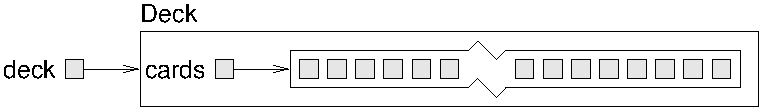
\includegraphics{figs/deckobject.pdf}
\end{center}

Here is a no-argument constructor that makes a 52-card deck and populates it with \java{Card}s:

\begin{code}
    public Deck() {
        this.cards = new Card[52];
        int index = 0;
        for (int suit = 0; suit <= 3; suit++) {
            for (int rank = 1; rank <= 13; rank++) {
                cards[index] = new Card(suit, rank);
                index++;
            }
        }
    }
\end{code}

This method is similar to \java{makeDeck};
we just changed the syntax to make it a constructor.
To invoke it, we use \java{new}:

\index{new}
\index{statement!new}

\begin{code}
    Deck deck = new Deck();
\end{code}

Now it makes sense to put the methods that pertain to \java{Deck}s in the \java{Deck} class definition.
Looking at the methods we have written so far, one obvious candidate is \java{printDeck} (Section~\ref{printdeck}).
Here's how it looks, rewritten to work with a \java{Deck}:
\index{printDeck}

\begin{code}
    public static void printDeck(Deck deck) {
        for (int i = 0; i < deck.cards.length; i++) {
            Card.printCard(deck.cards[i]);
        }
    }
\end{code}

One change is the type of the parameter, from \java{Card[]} to \java{Deck}.

The second change is that we can no longer use \java{deck.length} to get the length of the array, because \java{deck} is a \java{Deck} object now, not an array.
It contains an array, but it is not an array.
So we have to write \java{deck.cards.length} to extract the array from the \java{Deck} object and get the length of the array.

For the same reason, we have to use \java{deck.cards[i]} to access an element of the array, rather than just \java{deck[i]}.

The last change is that the invocation of \java{printCard} has to say explicitly that \java{printCard} is defined in the \java{Card} class.


\section{Shuffling}
\label{shuffle}
\index{shuffling}

For most card games you need to be able to shuffle the deck; that is, put the cards in a random order.
In Section~\ref{random} we saw how to generate random numbers, but it is not obvious how to use them to shuffle a deck.

One possibility is to model the way humans shuffle, which is usually by dividing the deck in two and then choosing alternately from each deck.
Since humans usually don't shuffle perfectly, after about 7 iterations the order of the deck is pretty well randomized.
But a computer program would have the annoying property of doing a perfect shuffle every time, which is not really very random.
In fact, after 8 perfect shuffles, you would find the deck back in the order you started in.
For more information, see \url{http://en.wikipedia.org/wiki/Faro_shuffle}.

A better shuffling algorithm is to traverse the deck one card at a time, and at each iteration choose two cards and swap them.

Here is an outline of how this algorithm works.
To sketch the program, I am using a combination of Java statements and English words that is sometimes called {\bf pseudocode}:

\index{pseudocode}

\begin{code}
    for (int i = 0; i < deck.cards.length; i++) {
        // choose a number between i and deck.cards.length-1
        // swap the ith card and the randomly-chosen card
    }
\end{code}

The nice thing about pseudocode is that it often makes it clear what methods you are going to need.
In this case, we need something like \java{randomInt}, which chooses a random integer between \java{low} and \java{high}, and \java{swapCards} which takes two indices and switches the cards at the indicated positions.

\index{random number}
\index{swapCards}
\index{reference}

This process---writing pseudocode first and then writing methods to make it work---is called {\bf top-down development} (see \url{http://en.wikipedia.org/wiki/Top-down_and_bottom-up_design}).

\index{program development}

\section{Selection sort algorithm}
\label{sorting}
\index{sorting}

Now that we have messed up the deck, we need a way to put it back in order.
There is an algorithm for sorting that is ironically similar to the algorithm for shuffling.
It's called {\bf selection sort} because it works by traversing the array repeatedly and selecting the lowest remaining card each time.

\index{selection sort}

During the first iteration we find the lowest card and swap it with the card in the 0th position.
During the \java{i}th, we find the lowest card to the right of \java{i} and swap it with the \java{i}th card.

Here is pseudocode for selection sort:

\begin{code}
    for (int i = 0; i < deck.cards.length; i++) {
        // find the lowest card at or to the right of i
        // swap the ith card and the lowest card
    }
\end{code}

Again, the pseudocode helps with the design of the {\bf helper methods}.
In this case we can use \java{swapCards} again, so we only need one new one, called \java{indexLowestCard}, that takes an array of cards and an index where it should start looking.

\index{helper method}
\index{method!helper}


\section{Subdecks}
\index{subdeck}

How should we represent a hand or some other subset of a full deck?
One possibility is to create a new class called \java{Hand}, which might extend \java{Deck}.
Another possibility, the one I will demonstrate, is to represent a hand with a \java{Deck} object with fewer than 52 cards.

We might want a method, \java{subdeck}, that takes a Deck and a range of indices, and that returns a new Deck that contains the specified subset of the cards:

\begin{code}
public static Deck subdeck(Deck deck, int low, int high) {
    Deck sub = new Deck(high-low+1);

    for (int i = 0; i<sub.cards.length; i++) {
        sub.cards[i] = deck.cards[low+i];
    }
    return sub;
}
\end{code}

The length of the subdeck is \java{high-low+1} because both the low card and high card are included.
This sort of computation can be confusing, and lead to ``off-by-one'' errors.
Drawing a picture is usually the best way to avoid them.

Because we provide an argument with \java{new}, the contructor that gets invoked will be the first one, which only allocates the array and doesn't allocate any cards.
Inside the \java{for} loop, the subdeck gets populated with copies of the references from the deck.

\index{constructor}
\index{overloading}

The following is a state diagram of a subdeck being created with the parameters \java{low=3} and \java{high=7}.
The result is a hand with 5 cards that are shared with the original deck, i.e., they are aliased.

\begin{center}
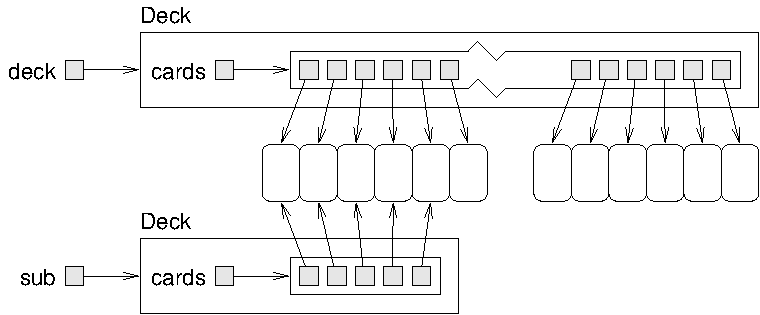
\includegraphics{figs/subdeck.pdf}
\end{center}

\index{aliasing}
\index{reference}

Aliasing is usually not generally a good idea, because changes in one subdeck are reflected in others, which is not the behavior you would expect from real cards and decks.
But if the cards are immutable, aliasing is less dangerous.
In this case, there is probably no reason ever to change the rank or suit of a card.
Instead we can create each card once and then treat it as an immutable object.
So for \java{Card}s aliasing is a reasonable choice.


\section{Shuffling and dealing}
\index{shuffling}
\index{dealing}

In Section~\ref{shuffle} I wrote pseudocode for a shuffling algorithm.
Assuming that we have a method called \java{shuffleDeck} that takes a deck as an argument and shuffles it, we can use it to deal hands:

\begin{code}
    Deck deck = new Deck();
    shuffleDeck(deck);

    Deck hand1 = subdeck(deck, 0, 4);
    Deck hand2 = subdeck(deck, 5, 9);
    Deck pack = subdeck(deck, 10, 51);
\end{code}

This code puts the first 5 cards in one hand, the next 5 cards in the other, and the rest into the pack.

When you thought about dealing, did you think we should give one card to each player in the round-robin style that is common in real card games?
I thought about it, but then realized that it is unnecessary for a computer program.
The round-robin convention is intended to mitigate imperfect shuffling and make it more difficult for the dealer to cheat.
Neither of these is an issue for a computer.

This example is a useful reminder of one of the dangers of engineering metaphors: sometimes we impose restrictions on computers that are unnecessary, or expect capabilities that are lacking, because we unthinkingly extend a metaphor past its breaking point.


\section{Insertion sort algotihm}

TODO


\section{Merge sort algorithm}
\label{mergesort}
\index{efficiency}
\index{sorting}
\index{mergesort}

In Section~\ref{sorting}, we saw a simple sorting algorithm that turns out not to be very efficient.
To sort $n$ items, it has to traverse the array $n$ times, and each traversal takes an amount of time that is proportional to $n$.
The total time, therefore, is proportional to $n^2$.

In this section I sketch a more efficient algorithm called {\bf mergesort}.
To sort $n$ items, mergesort takes time proportional to $n \log n$.
That may not seem impressive, but as $n$ gets big, the difference between $n^2$ and $n \log n$ can be enormous.
Try out a few values of $n$ and see.

The basic idea behind mergesort is this: if you have two subdecks, each of which has been sorted, it is easy (and fast) to merge them into a single, sorted deck.
Try this out with a deck of cards:

\begin{enumerate}

\item Form two subdecks with about 10 cards each and sort them so that when they are face up the lowest cards are on top.
Place both decks face up in front of you.

\item Compare the top card from each deck and choose the lower one.
Flip it over and add it to the merged deck.

\item Repeat step two until one of the decks is empty.
Then take the remaining cards and add them to the merged deck.

\end{enumerate}

The result should be a single sorted deck.
Here's what this looks like in pseudocode:

\begin{code}
public static Deck merge(Deck d1, Deck d2) {
    // create a new deck big enough for all the cards
    Deck result = new Deck(d1.cards.length + d2.cards.length);

    // use the index i to keep track of where we are in
    // the first deck, and the index j for the second deck
    int i = 0;
    int j = 0;

    // the index k traverses the result deck
    for (int k = 0; k < result.cards.length; k++) {

        // if d1 is empty, d2 wins; if d2 is empty, d1 wins;
        // otherwise, compare the two cards

        // add the winner to the new deck
    }
    return result;
}
\end{code}

The best way to test \java{merge} is to build and shuffle a deck, use subdeck to form two (small) hands, and then use the sort routine from the previous chapter to sort the two halves.
Then you can pass the two halves to \java{merge} to see if it works.

\index{testing}

If you can get that working, try a simple implementation of
\java{mergeSort}:

\begin{code}
public static Deck mergeSort(Deck deck) {
    // find the midpoint of the deck
    // divide the deck into two subdecks
    // sort the subdecks using sortDeck
    // merge the two halves and return the result
}
\end{code}

Then, if you get that working, the real fun begins!  The magical thing about mergesort is that it is recursive.
At the point where you sort the subdecks, why should you invoke the old, slow version of {\tt sort}?
Why not invoke the spiffy new \java{mergeSort} you are in the process of writing?

\index{recursion}

Not only is that a good idea, it is {\em necessary} to achieve the performance advantage I promised.
But to make it work you have to have a base case; otherwise it recurses forever.
A simple base case is a subdeck with 0 or 1 cards.
If {\tt mergesort} receives such a small subdeck, it can return it unmodified, since it is already sorted.

The recursive version of \java{mergesort} should look something like this:

\begin{code}
public static Deck mergeSort(Deck deck) {
    // if the deck is 0 or 1 cards, return it

    // find the midpoint of the deck
    // divide the deck into two subdecks
    // sort the subdecks using mergesort
    // merge the two halves and return the result
}
\end{code}

As usual, there are two ways to think about recursive programs: you can think through the entire flow of execution, or you can make the ``leap of faith'' (see Section~\ref{leap of faith}).
I have constructed this example to encourage you to make the leap of faith.

\index{leap of faith}

When you use \java{sortDeck} to sort the subdecks, you don't feel compelled to follow the flow of execution, right?
You just assume it works because you already debugged it.
Well, all you did to make \java{mergeSort} recursive was replace one sorting algorithm with another.
There is no reason to read the program differently.

Actually, you have to give some thought to getting the base case right and making sure that you reach it eventually, but other than that, writing the recursive version should be no problem.
Good luck!


\section{Vocabulary}

\begin{description}

\term{pseudocode}
A way of designing programs by writing rough drafts in a combination of English and Java.

\term{helper method}
Often a small method that does not do anything enormously useful by itself, but which helps another, more useful method.

\term{abstract parameter}
A set of parameters that act together as a single parameter.

\term{abstraction}
The process of interpreting a program (or anything else) at a higher level than what is literally represented by the code.

\end{description}


\section{Exercises}


\begin{exercise}
The goal of this exercise is to implement the shuffling and sorting algorithms from this chapter.

\begin{enumerate}

\item Download the code from this chapter from \url{http://thinkapjava.com/code/Card2.java} and import it into your development environment.
I have provided outlines for the methods you will write, so the program should compile.
But when it runs it prints messages indicating that the empty methods are not working.
When you fill them in correctly, the messages should go away.

\item If you did Exercise~\ref{ex.randint}, you already wrote \java{randomInt}.
Otherwise, write it now and add code to test it.

\item Write a method called \java{swapCards} that takes a deck (array of cards) and two indices, and that switches the cards at those two locations.

HINT: it should switch references, not the contents of the objects.
This is faster; also, it correctly handles the case where cards are aliased.

\item Write a method called \java{shuffleDeck} that uses the algorithm in Section~\ref{shuffle}.
You might want to use the \java{randomInt} method from Exercise~\ref{ex.randint}.

\item Write a method called \java{indexLowestCard} that uses the \java{compareCard} method to find the lowest card in a given range of the deck (from \java{lowIndex} to \java{highIndex}, including both).

\item Write a method called \java{sortDeck} that arranges a deck of cards from lowest to highest.

\item Using the pseudocode in Section~\ref{mergesort}, write the method called \java{merge}.
Be sure to test it before trying to use it as part of a \java{mergeSort}.

\item Write the simple version of \java{mergeSort}, the one that divides the deck in half, uses \java{sortDeck} to sort the two halves, and uses \java{merge} to create a new, fully-sorted deck.

\item Write the fully recursive version of \java{mergeSort}.
Remember that \java{sortDeck} is a modifier and \java{mergeSort} is a function, which means that they get invoked differently:

\begin{code}
sortDeck(deck);              // modifies existing deck
deck = mergeSort(deck);      // replaces old deck with new
\end{code}

\end{enumerate}
\end{exercise}


\end{document}
